\chapter{背景知识}
\label{chap:pre}
为了保持文章的完整性,这一章我们介绍一些与MR成像和MRF重建相关的预备知识。

\section{MRI基本原理}
\label{sec:mr}
在这一小节,我们有简单回顾一下MR成像的基本过程和数学建模,这有利于我们加深对压缩感知MRI的理解。更详细的MR成像原理请参考文献\cite{mrireview,2009nmr,haacke1999magnetic}。

\subsection{数学建模}
\label{sec:mrimodel}
核磁共振成像可以非侵入性地获取人体内组织的图像,成像分辨率高,并且没有暴露在辐射中的危险。它主要利用了磁共振原理,反应了磁化粒子(主要是氢原子)和磁场的交互作用。MR成像系统如图\ref{fig:system}所示。
\begin{figure}[htbp]
\centering
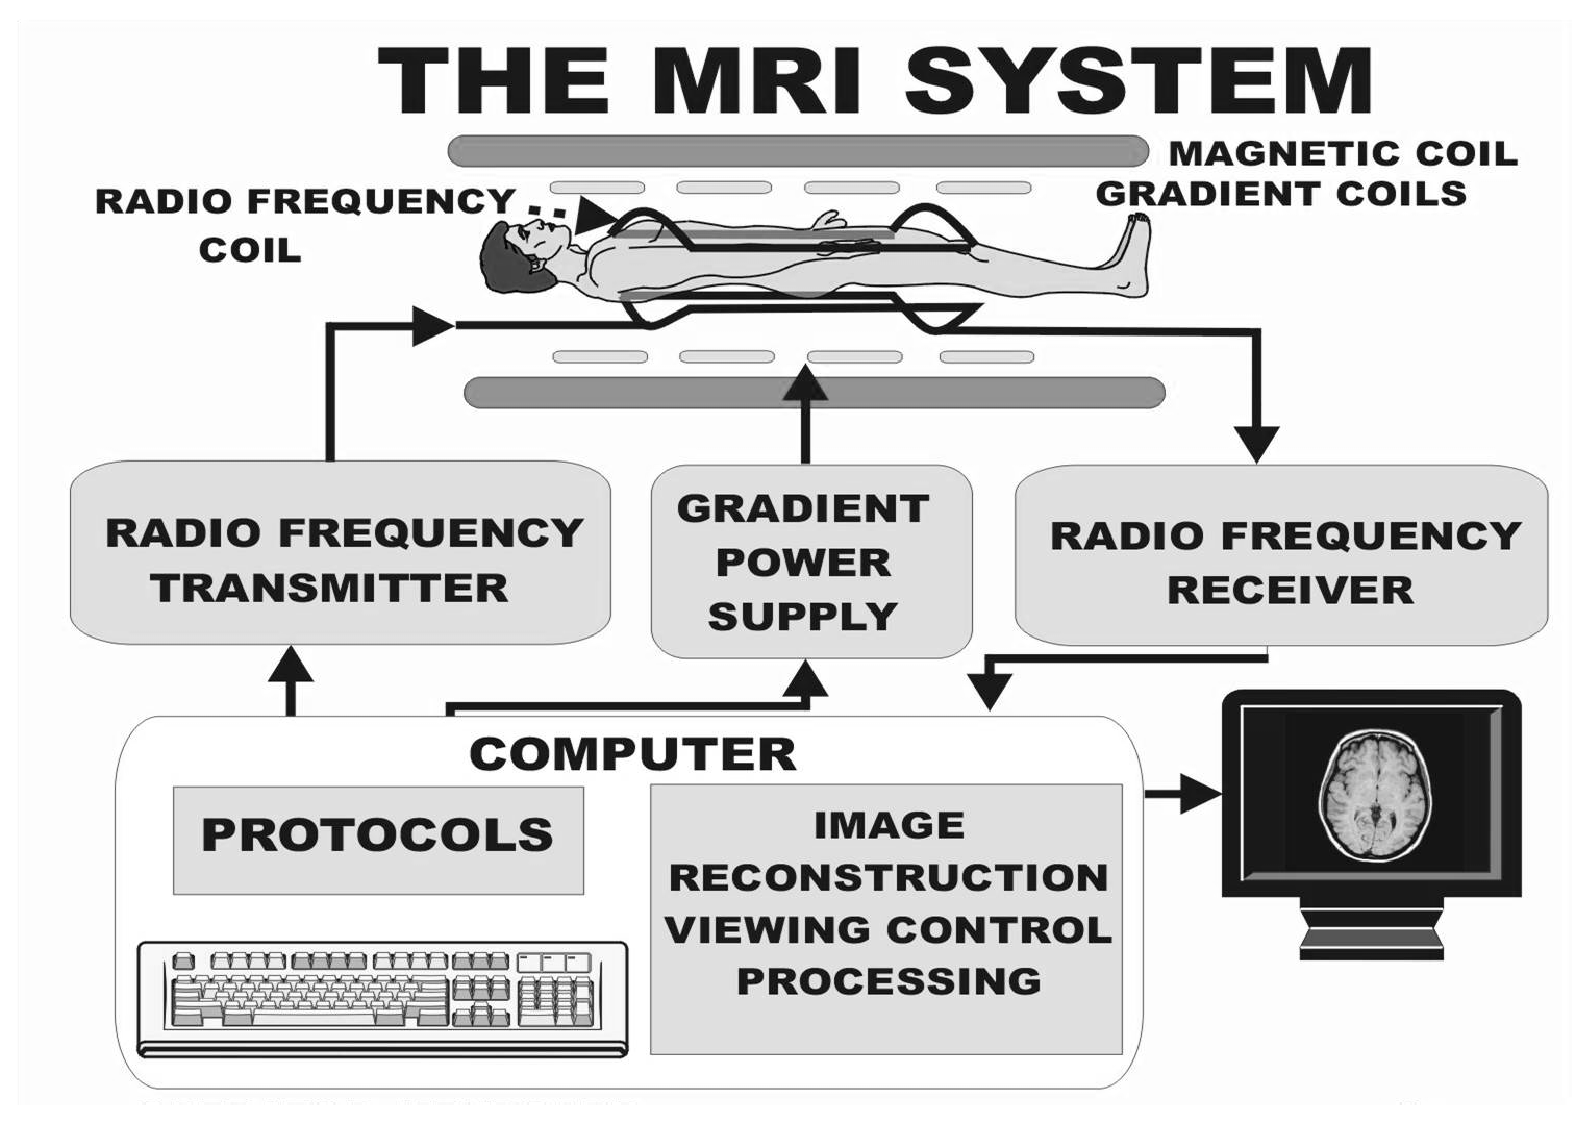
\includegraphics[width=0.8\textwidth]{img/intro/system.eps}
\caption{MR成像系统。此图来自于文献\cite{sprawls2000magnetic}。}
\label{fig:system}
\end{figure}
其中有三个磁场的概念最为重要,第一个是主磁场(the main magnetic field),由主磁场线圈(magnetic coil)产生,如图\ref{fig:main}所示。
\begin{figure}[htbp]
\centering
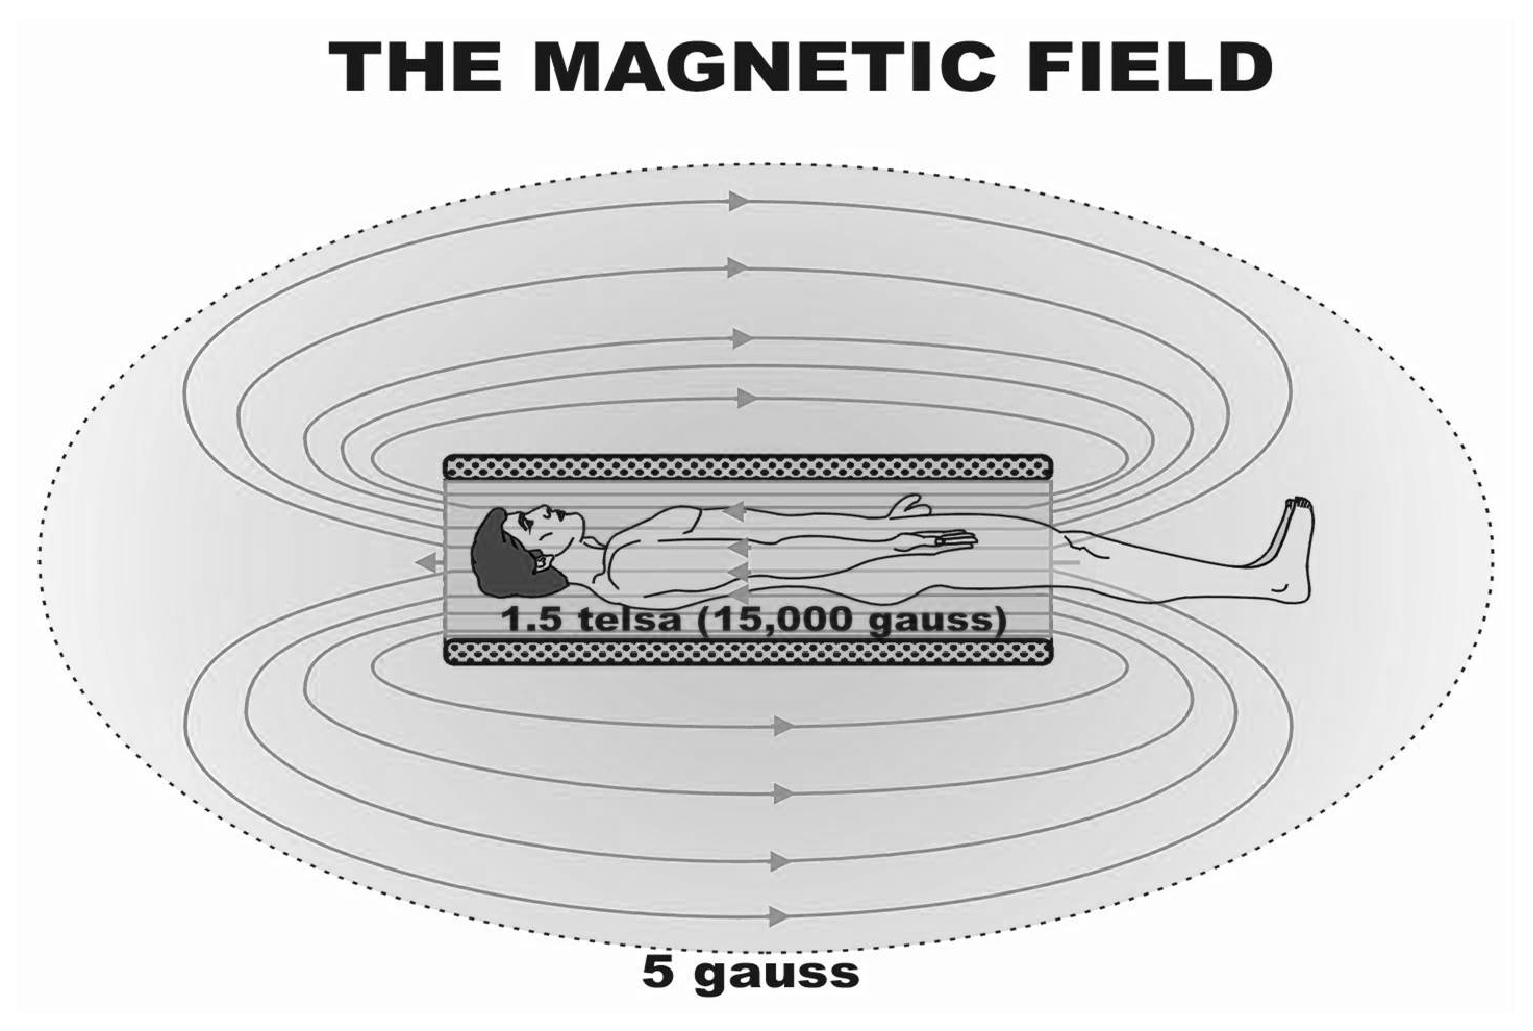
\includegraphics[width=0.8\textwidth]{img/intro/main.eps}
\caption{MR主磁场。此图来自于文献\cite{sprawls2000magnetic}。}
\label{fig:main}
\end{figure}
主磁场是大小和方向都不变的静磁场,一般约定为$z$轴方向,记为$\mathrm{\textbf{B}}_0$。第二个磁场是射频场(radio frequency,RF),由射频线圈(radio frenquency coil)产生,如图\ref{fig:rf}所示。
\begin{figure}[htbp]
\centering
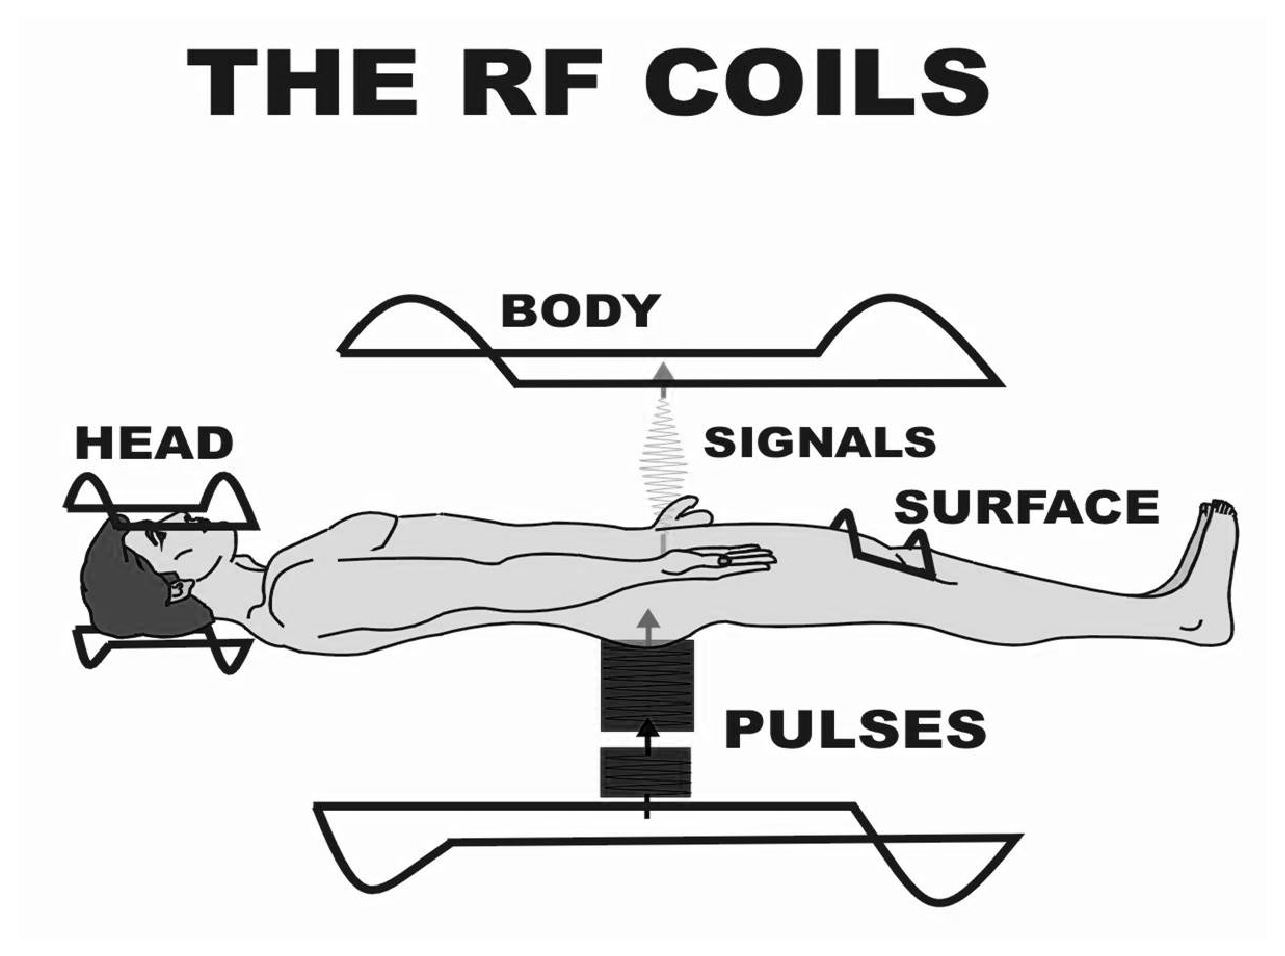
\includegraphics[width=0.8\textwidth]{img/intro/rf.eps}
\caption{MR射频场。此图来自于文献\cite{sprawls2000magnetic}。}
\label{fig:rf}
\end{figure}
射频场是周期性变化的磁场,方向与主磁场垂直,记为$\mathrm{\textbf{B}}_1$。其作用是激活待成像粒子,使之发生共振,用于之后的成像。第三个磁场是梯度场(gradient fields),由梯度线圈产生(gradient coils),如图\ref{fig:gradient}所示。
\begin{figure}[htbp]
\centering
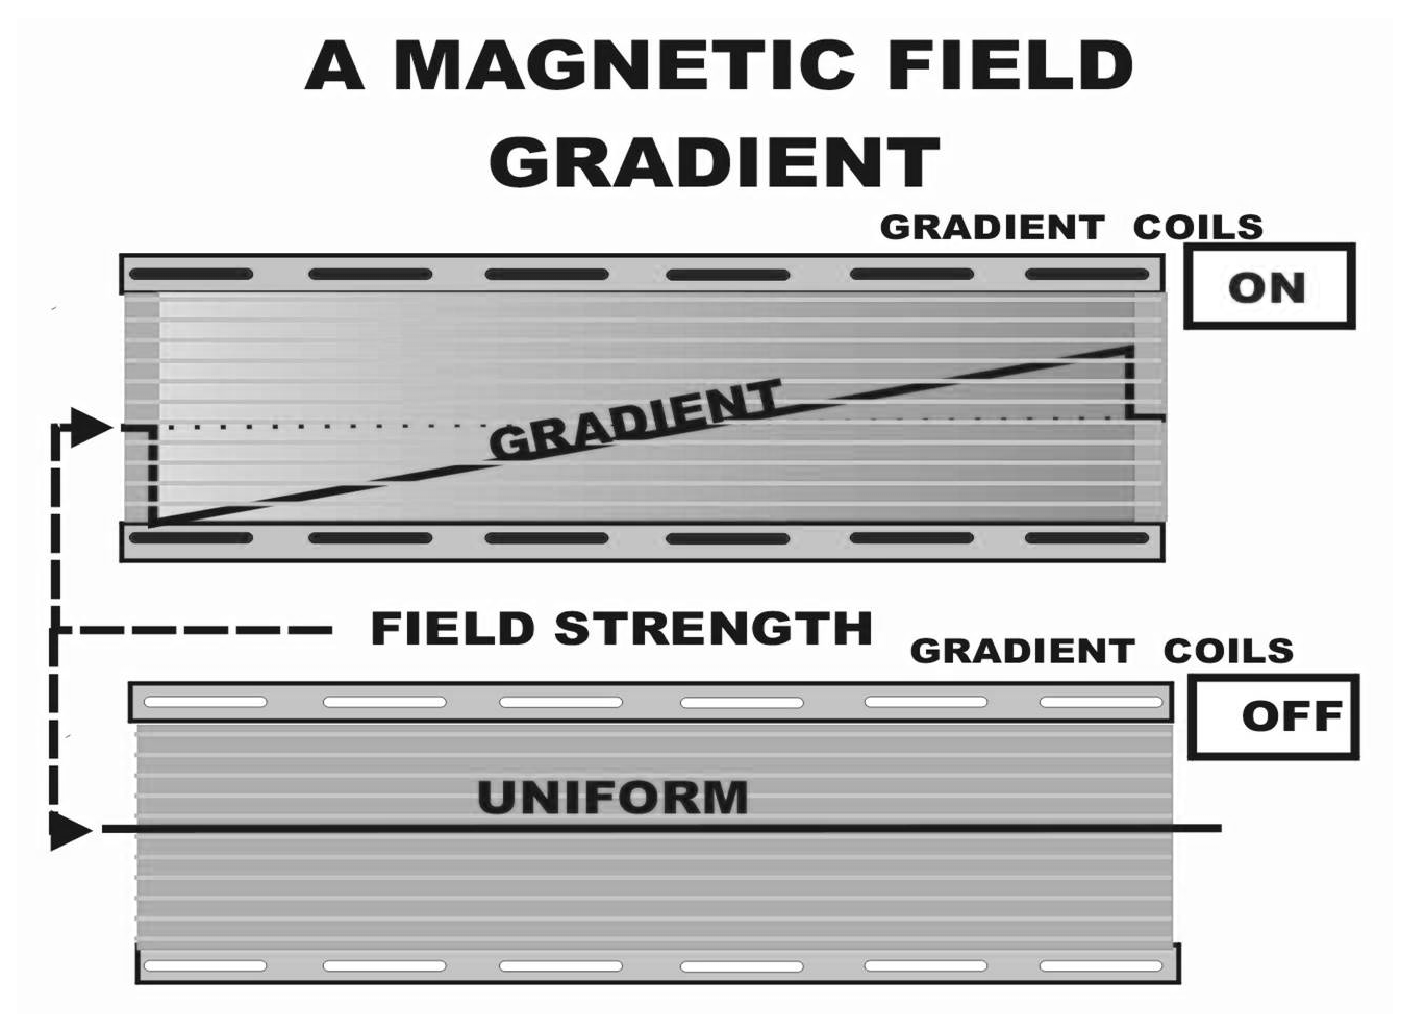
\includegraphics[width=0.8\textwidth]{img/intro/gradient.eps}
\caption{MR梯度场。此图来自于文献\cite{sprawls2000magnetic}。}
\label{fig:gradient}
\end{figure}
梯度场的方向与主磁场平行,且大小随着空间位置的变化而变化。梯度场的作用是使得主磁场的大小发生改变,在$x$,$y$或者$z$方向上产生一个梯度,用于之后的成像过程。

成像前,所有待成像原子都做无规则的运动,其合磁场为\textbf{0}。开始成像时,打开主磁场$\mathrm{\textbf{B}}_0$。一段时间后,所有待成像的原子会被主磁场磁化,进入热平衡状态,产生一个平行于主磁场方向的磁动量$\mathrm{\textbf{M}}$。然后打开射频场,于此同时打开预先设定好的梯度场,这样会使得待成像原子产生共振,处于激发态。宏观上来看,$\mathrm{\textbf{M}}$会绕着磁场$\mathrm{\textbf{B}}_0$以Larmor频率$\omega$旋转:
\begin{equation}
	\omega=-\gamma|\mathrm{\textbf{B}}|.
\end{equation}
其中$\gamma$是旋磁率(常数)。这个过程被成为进动(procession)。可以看出,磁动量的Larmor频率的大小与其所处的磁场大小成正比。这里的磁场$\mathrm{\textbf{B}}$由四部分构成,分别为主磁场$\mathrm{\textbf{B}}_0$和三个方向的梯度场$G_x(t)$, $G_y(t)$和$G_z(t)$:
\begin{equation}
	\mathrm{\textbf{B}}(x,y,z,t)=\mathrm{\textbf{B}}_0+x G_x(t)+y G_y(t)+z G_z(t).
\end{equation}
 其中主磁场的大小和方向不变,而梯度场是大小随时间和空间变化的磁场,决定了磁场$\mathrm{\textbf{B}}$的大小和方向。记梯度场向量为$\mathrm{\textbf{G}}(t)=(G_x(t),G_y(t),G_z(t))$。
 
 $\mathrm{\textbf{M}}$被射频场从热平衡态激发之后,逐渐偏离主磁场,并产生一个垂直与主磁场方向的磁化$M_{xy}$。我们将$\mathrm{\textbf{M}}$偏离主磁场的角度,$\mathrm{\textbf{M}}$即与$z$轴的夹角称为偏转角(flip angle),记为$\alpha$,将$\mathrm{\textbf{M}}$与$x$轴的夹角称为相位角(phase angle),记为$\phi$,将磁动量在$x$,$y$,$z$处,$t$时刻的密度(density)记为$m(x,y,z,t)$, 则进动的角度或者相位累积为:
 \begin{equation}
 \begin{aligned}
 	 \phi(x,y,z,t)&=-\int_{t'=0}^t \gamma|\mathrm{\textbf{B}}(x,y,z,t')|\mathrm{d}t'\\
 	&=\omega_0t-2\pi(xk_x(t)+yk_y(t)+zk_z(t)),
 \end{aligned}
 \end{equation}
其中
\begin{equation}
	\omega_0=-\gamma|\mathrm{\textbf{B}}_0|,
\end{equation}
\begin{equation}
\begin{aligned}
	k_x(t)=\frac{\gamma}{2\pi}\int_{t'=0}^t G_x(t')\mathrm{d}t',\\
	k_y(t)=\frac{\gamma}{2\pi}\int_{t'=0}^t G_y(t')\mathrm{d}t',\\
	k_z(t)=\frac{\gamma}{2\pi}\int_{t'=0}^t G_z(t')\mathrm{d}t'.
\end{aligned}
\end{equation}

通过上面的方程可以看出,位置$x$,$y$,$z$相对于初始位置的累积旋进角度等于位置向量$\mathrm{\textbf{r}}=(x,y,z)$与向量$\mathrm{\textbf{k}}(t)=(k_x(t),k_y(t),k_z(t))$的内积的$-2\pi$倍。
我们定义$\mathrm{\textbf{k}}(t)$为k-space。k-space是MR成像中最基本的概念,在之后的章节也会用到。有了相位,我们就可以计算任意时刻在位置$\mathrm{\textbf{r}}$的磁场密度:
\begin{equation}
	\begin{aligned}
		m_{xy}(x,y,z,t)&=m_{xy}(x,y,z,0)e^{i\phi(x,y,z,t)} \\
&=m_{xy}(x,y,z,0)e^{i\omega_0t}e^{-2\pi i(xk_x(t)+yk_y(t)+zk_z(t))}.
	\end{aligned}
\end{equation}
这里$m_{xy}=m_x+im_y$。然后我们对视野内(field of view,FOV)所有原子的磁场密度进行积分
\begin{equation}
	\begin{aligned}
		M_{xy}&=\int_{\mathrm{FOV}}m_{xy}(x,y,z,t)\mathrm{d}\mathrm{\textbf{r}} \\
&=e^{i\omega_0t}\int_{\mathrm{FOV}}m_{xy}(x,y,z,0)e^{-2\pi i(xk_x(t)+yk_y(t)+zk_z(t))}\mathrm{d}\mathrm{\textbf{r}}.
	\end{aligned}
\end{equation}
我们记$x(\mathrm{\textbf{r}})=m_{xy}(x,y,z,0)$并且去掉检测阶段的$e^{i\omega_0t}$,我的得到最终MRI信号:
\begin{equation}
	b(\mathrm{\textbf{k}}(t)) = \int_{\mathrm{FOV}}x(\mathrm{\textbf{r}})e^{-2\pi i\mathrm{\textbf{k}}(t) \cdot \mathrm{\textbf{r}}}\mathrm{d}\mathrm{\textbf{r}}.
	\label{equ:mri}
\end{equation}
从方程(\ref{equ:mri})中可以看出,MRI信号大小与图像的Fourier变换成正比。由于测量得到的信号是Fourier域的数据,因此要最终的图像$x(\mathrm{\textbf{r}})$,需要从采集到的数据$b(\mathrm{\textbf{k}}(t))$中恢复出$x(\mathrm{\textbf{r}})$。

\subsection{图像重建}
我们的目标是从采集到的数据$b(\mathrm{\textbf{k}}(t))$中恢复出$x(\mathrm{\textbf{r}})$。首先,我们假设以下两点。第一,采集得到的k-space数据是有限的;第二,测量过程是带有噪声的。因此方程(\ref{equ:mri})可以写为:
\begin{equation}
	b(\mathrm{\textbf{k}}_m) = \int_{\mathrm{FOV}} x(r)e^{-2\pi i \mathrm{\textbf{k}}_m \cdot \mathrm{\textbf{r}}}\mathrm{d}\mathrm{\textbf{r}} + \epsilon(\mathrm{\textbf{k}}_m), m=1,...,M.
	\label{equ:mrinoise}
\end{equation}
由于$b(\mathrm{\textbf{r}})$为连续形式,而我们只有有限个k-space采样点,因此这个重建过程是病态的。Nyquist采样定理表明,如果要精确地重建出信号,采样率需要达到信号最高频率的两倍以上。这我们假设采样达到了Nyquist采样定理的要求,我们称之为全采样。为了将图像重建出来,我们可以对这个病态问题提出合理的假设。这里我们假设,$x(\mathrm{\textbf{r}})$属于有限维空间,则$b(\mathrm{\textbf{r}})$可以用这个空间的一组基来表示:
\begin{equation}
	b(\mathrm{\textbf{r}})=\sum_{n=1}^N b_n\psi_n(\mathrm{\textbf{r}}).
	\label{equ:linear}
\end{equation}
这里$\psi_{n}(\mathrm{\textbf{r}}), n=1,...N$为基函数,N为空间的维度。基函数的选择有很多种,一般来说,可以取$\psi(\mathrm{\textbf{r}})$为Dirac函数或者矩形方程。将方程(\ref{equ:linear})和$\psi(\mathrm{\textbf{r}})$带入方程(\ref{equ:mrinoise})得到:
\begin{equation}
	b(\mathrm{\textbf{k}}_m) = \sum_{n=1}^N A_{m,n}b_n + \epsilon(\mathrm{\textbf{k}}_m), m=1,...,M.
\end{equation}
这里$A_{m,n}=e^{-2\pi i\mathrm{\textbf{k}}_m\mathrm{\textbf{r}}_n}\Psi(\mathrm{\textbf{k}}_m)$,$\Psi(\mathrm{\textbf{k}}_m)$为$\psi(\mathrm{\textbf{r}})$在$\mathrm{\textbf{k}}_m$点的Fourier变换。将上式写成矩阵形式则为:
\begin{equation}
	b=Ax+\epsilon,
	\label{equ:matrix}
\end{equation}
其中$b\in \mathbb{C}^M$为测量得到的数据,$A\in \mathbb{C}^{M\times N}$为测量矩阵,$x\in \mathbb{C}^N$为待重建图像,$\epsilon \in \mathbb{C}^N$为噪声。

\subsection{采样轨迹}
由上一部分可以知道,测量矩阵$A$取决于数据在k-space的采样轨迹$\mathrm{\textbf{k}}$和基函数$\psi(\mathrm{\textbf{r}})$的选择。比如,当$\psi(\mathrm{\textbf{r}})$为Dirac函数,$M=N$并且所有采样点都在均匀Cartetian的网格上时,测量矩阵$A$退化为Fourier变换矩阵。这时,方程(\ref{equ:matrix})可以通过快速Fourier变换(FFT)求解。

一般而言,如果测量矩阵$A$是列满秩的,即$M\geq N$,方程(\ref{equ:matrix})可以由最小二乘法(least square)求解
\begin{equation}
	\hat{x} = \argmin_x \|Ax-b\|^2_2.
	\label{equ:ls}
\end{equation}
方程(\ref{equ:ls})的解为:
\begin{equation}
	\hat{x} = (A^HA)^{-1}A^Hb.
	\label{equ:lss}
\end{equation}
其中,$A^H$为$A$的共轭转置。当$M\geq N$时,采样点的个数大于图像像素点的个数。由于MR成像速度慢,采集过多的数据会导致成像时间增长。因此在实际应用中,如平行成像、压缩感知等,通常是减少采样的个数来加快成像速度,即$M<N$,这时方程(\ref{equ:ls})则变为病态问题。

在MR成像中,采样轨迹是通过调整梯度场$G_x$,$G_y$和$G_z$的大小和方向来实现的。在理想情况下,我们希望整个k-space可以被一条光滑的采样轨迹所覆盖。但在实际情况中,由于信号的衰减和主磁场$\mathrm{\textbf{B}}_0$的非均匀,我们一般需要多条采样轨迹来覆盖k-space。这些采样轨迹合在一起称为采样模式。在第\ref{sec:csmri}小节中我们介绍过,MRI中的采样模式可以分为Cartesian采样和非Cartesian两大类。其中Cartesian采样计算简便,在临床中应用最为广泛;而非Cartesian的采样方式,如径向采样和螺旋采样可以达到更高的下采样率,但是计算比Cartesian采样繁琐。

\subsection{成像序列}
在这一节中我们介绍MR中常用的成像序列。在小节\ref{sec:mrimodel}中我们提到,当射频场打开之后,磁化$\mathrm{\textbf{M}}$发生共振激发,沿着主磁场方向进动。当射频场关闭之后,磁化$\mathrm{\textbf{M}}$会从激发态慢慢恢复到热平衡态,这一过程成为驰豫(relaxation)。我们将热平衡态的磁化大小记为$\mathrm{\textbf{M}}_0$,磁化$\mathrm{\textbf{M}}$的垂直分量记为$M_z$,水平分量记为$M_{xy}$。驰豫的过程即为$M_z$慢慢恢复而$M_{xy}$逐渐消失的过程。则根据方向的不同,我们将驰豫分为纵向驰豫和横向驰豫,他们满足以下Bloch方程\cite{bloch}:
\begin{equation}
\begin{aligned}
	&M_z(t)=\mathrm{\textbf{M}}_0(1-e^{-t/T_1}),\\
	&M_{xy}(t)=\mathrm{\textbf{M}}_0e^{-t/T_2}.
\end{aligned}
\end{equation}
其中$T_1$为纵向弛豫时间,是$M_z$恢复到63\%$\mathrm{\textbf{M}}_0$所需要的时间;$T_2$是横向驰豫时间,是$M_{xy}$损失为原来的37\%所需的时间。这里$T_1$和$T_2$是物质的固有属性,也是MR图像中对比度的主要来源。图\ref{fig:t1t2}展示了横向驰豫和纵向驰豫的过程。$T_1$和$T_2$在定量MR分析中有着重要的作用,这一点我们后面再介绍。

\begin{figure}[htbp]
\centering
\subfigure[横向驰豫]{
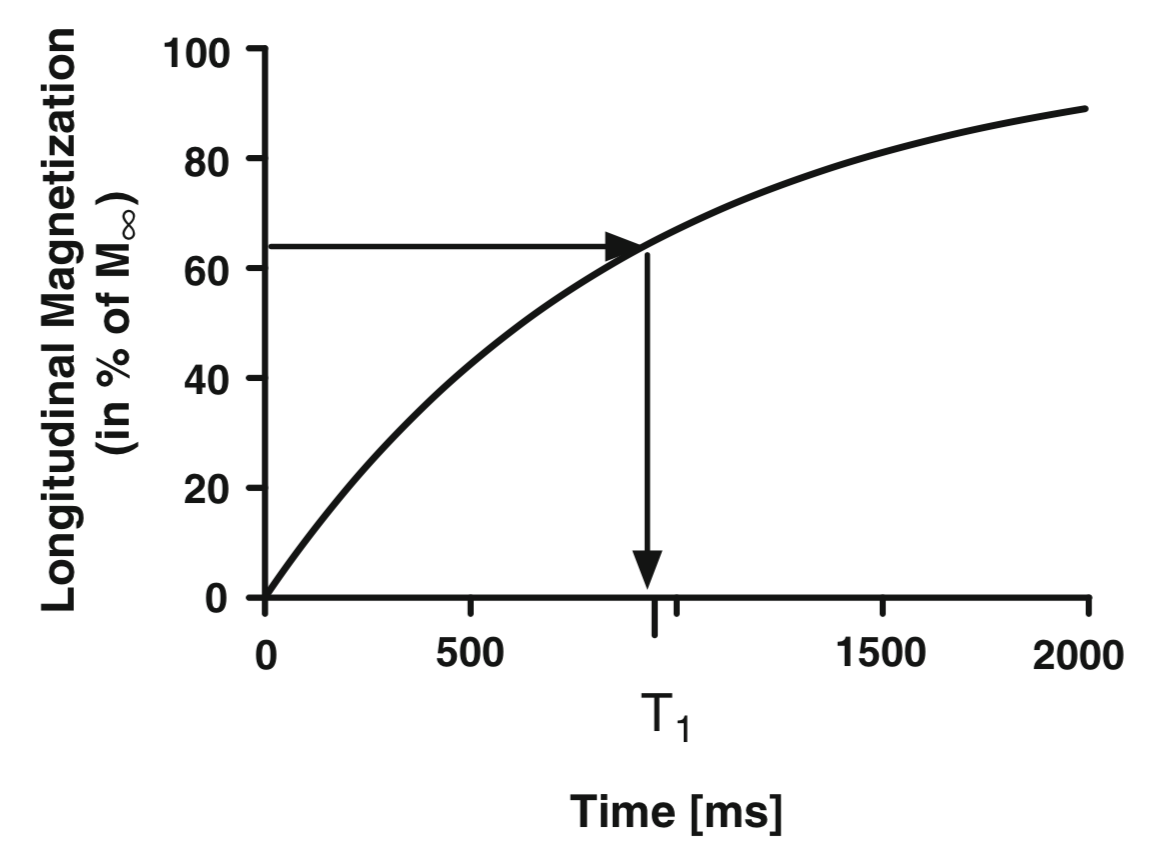
\includegraphics[width=3in]{img/intro/t1decay.png}
}
\subfigure[纵向驰豫]{
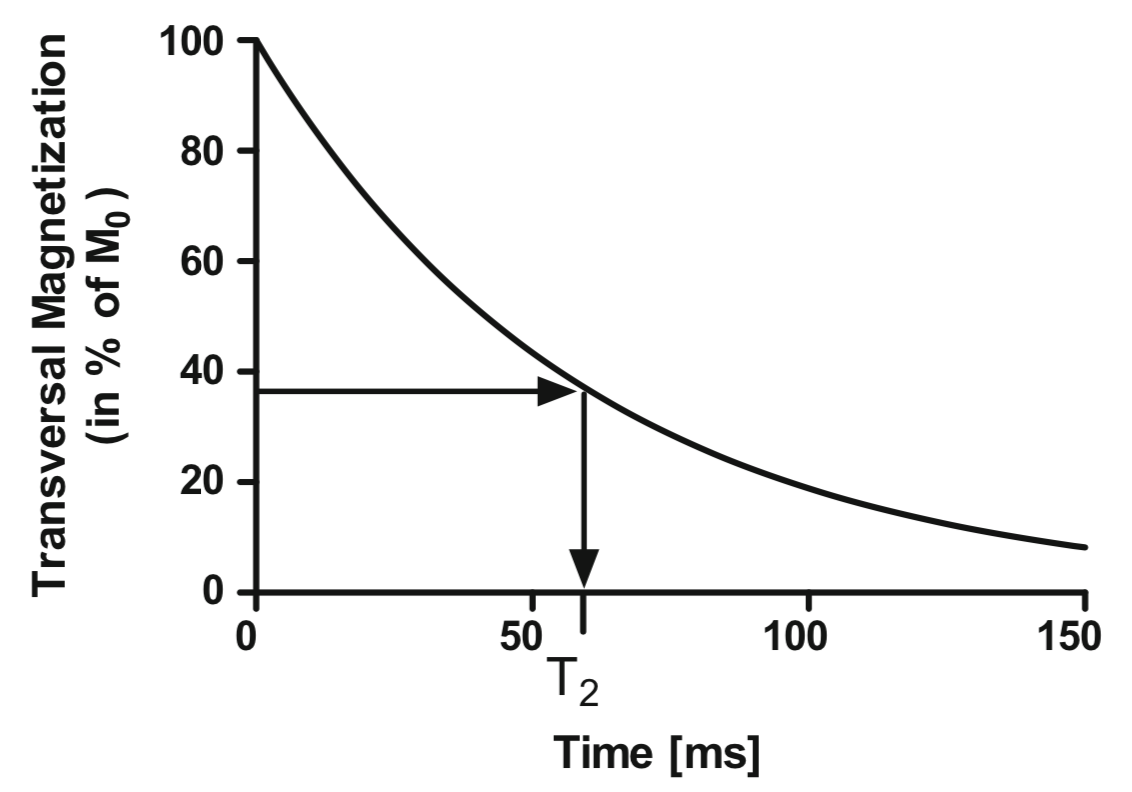
\includegraphics[width=3in]{img/intro/t2decay.png}
}
\centering
\caption{横向驰豫(a)与纵向驰豫(b)。此图来自文献\cite{haidekker2013medical}。}
\label{fig:t1t2}
\end{figure}

前面我们介绍了射频场和梯度场在MR成像的作用,而MR序列即为不同射频脉冲序列和梯度脉冲序列的特定设置,每个不同的MR序列都会影响最终所成图像。MR中常用的序列有两大类,一类是自旋回波序列(spin echo, SE),另一类是梯度回波序列(gradient echo, GE)。

自旋回波是MR成像中的基本序列,也是最常用的序列。自旋回波的过程如图\ref{fig:se}所示。其中回波时间(echo time, $T_E$)是90$^\circ$射频脉冲打开到收到回波的时间。自旋回波的特点是在$T_E/2$时刻加入了180$^\circ$的射频脉冲,使得磁化反向聚焦从而产生回波。
\begin{figure}[htbp]
\centerline{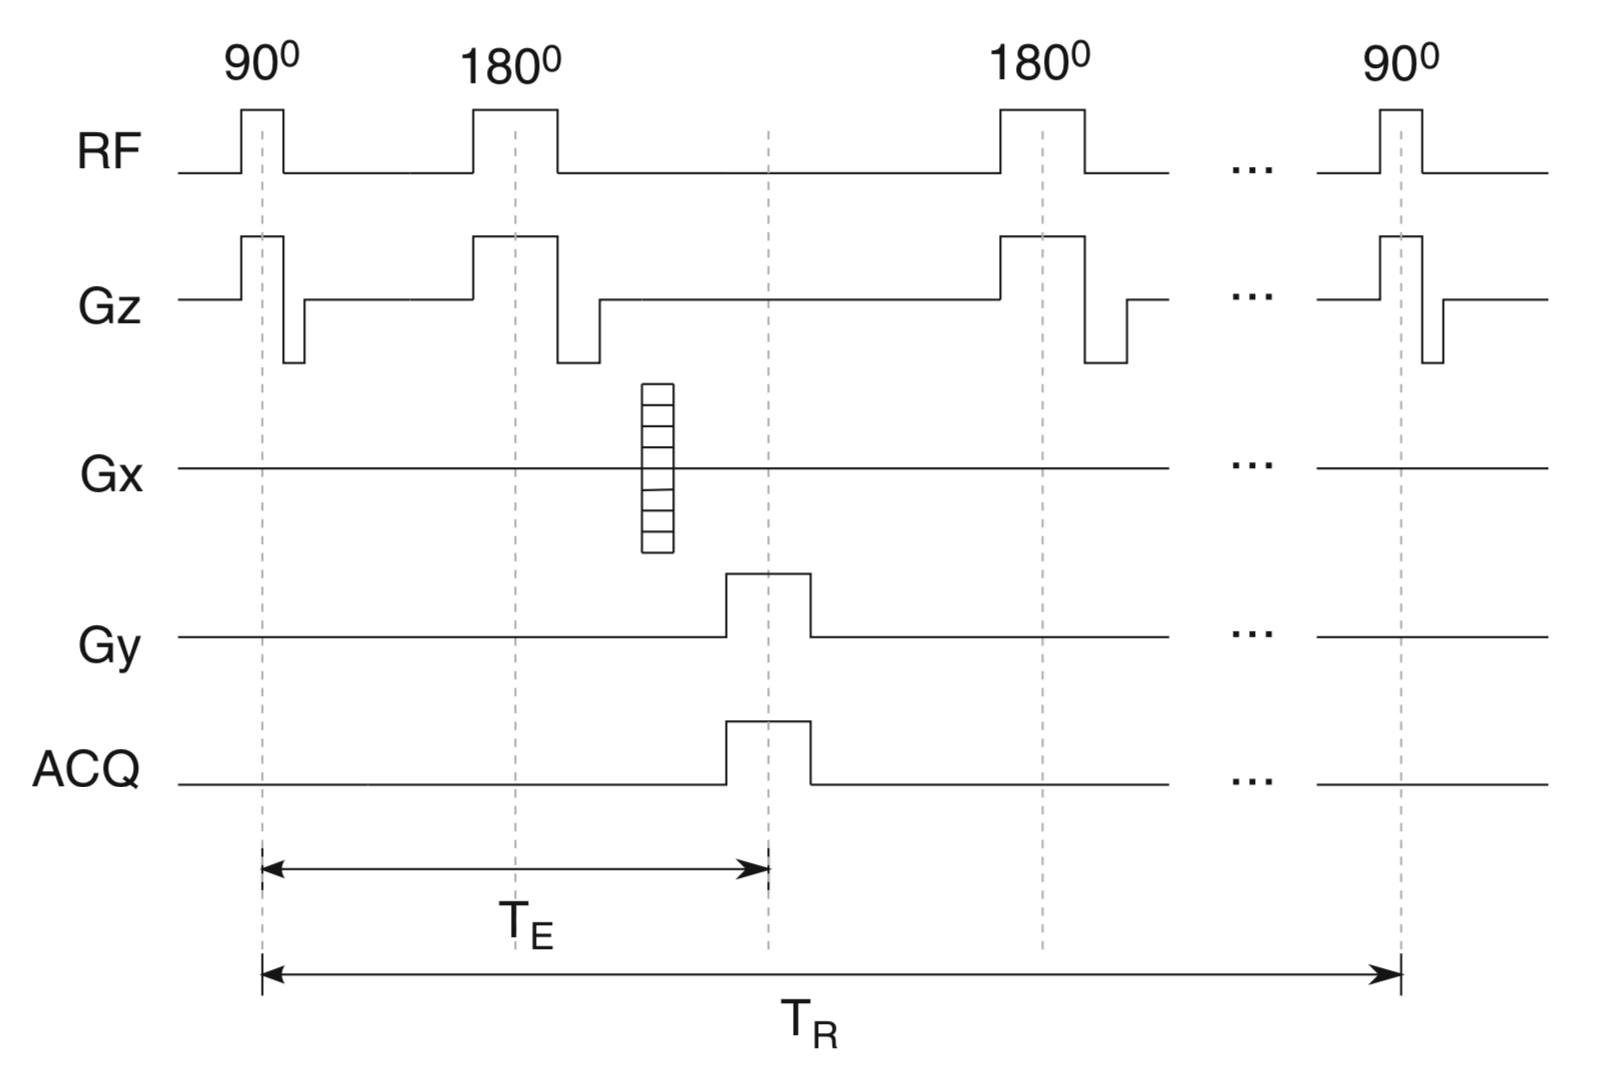
\includegraphics[width=0.9\textwidth]{img/intro/se.png}}
\caption{自旋回波序列。此图来自文献\cite{haidekker2013medical}。}
\label{fig:se}
\end{figure}
而梯度回波序列与自旋回波不同,它是靠梯度场的反向来达成聚焦从而产生回波。梯度回波的过程如图\ref{fig:ge}所示。其中,重复时间(repetion time, $T_R$)是连续两个射频脉冲的间隔时间,即序列的重复时间。
\begin{figure}[htbp]
\centerline{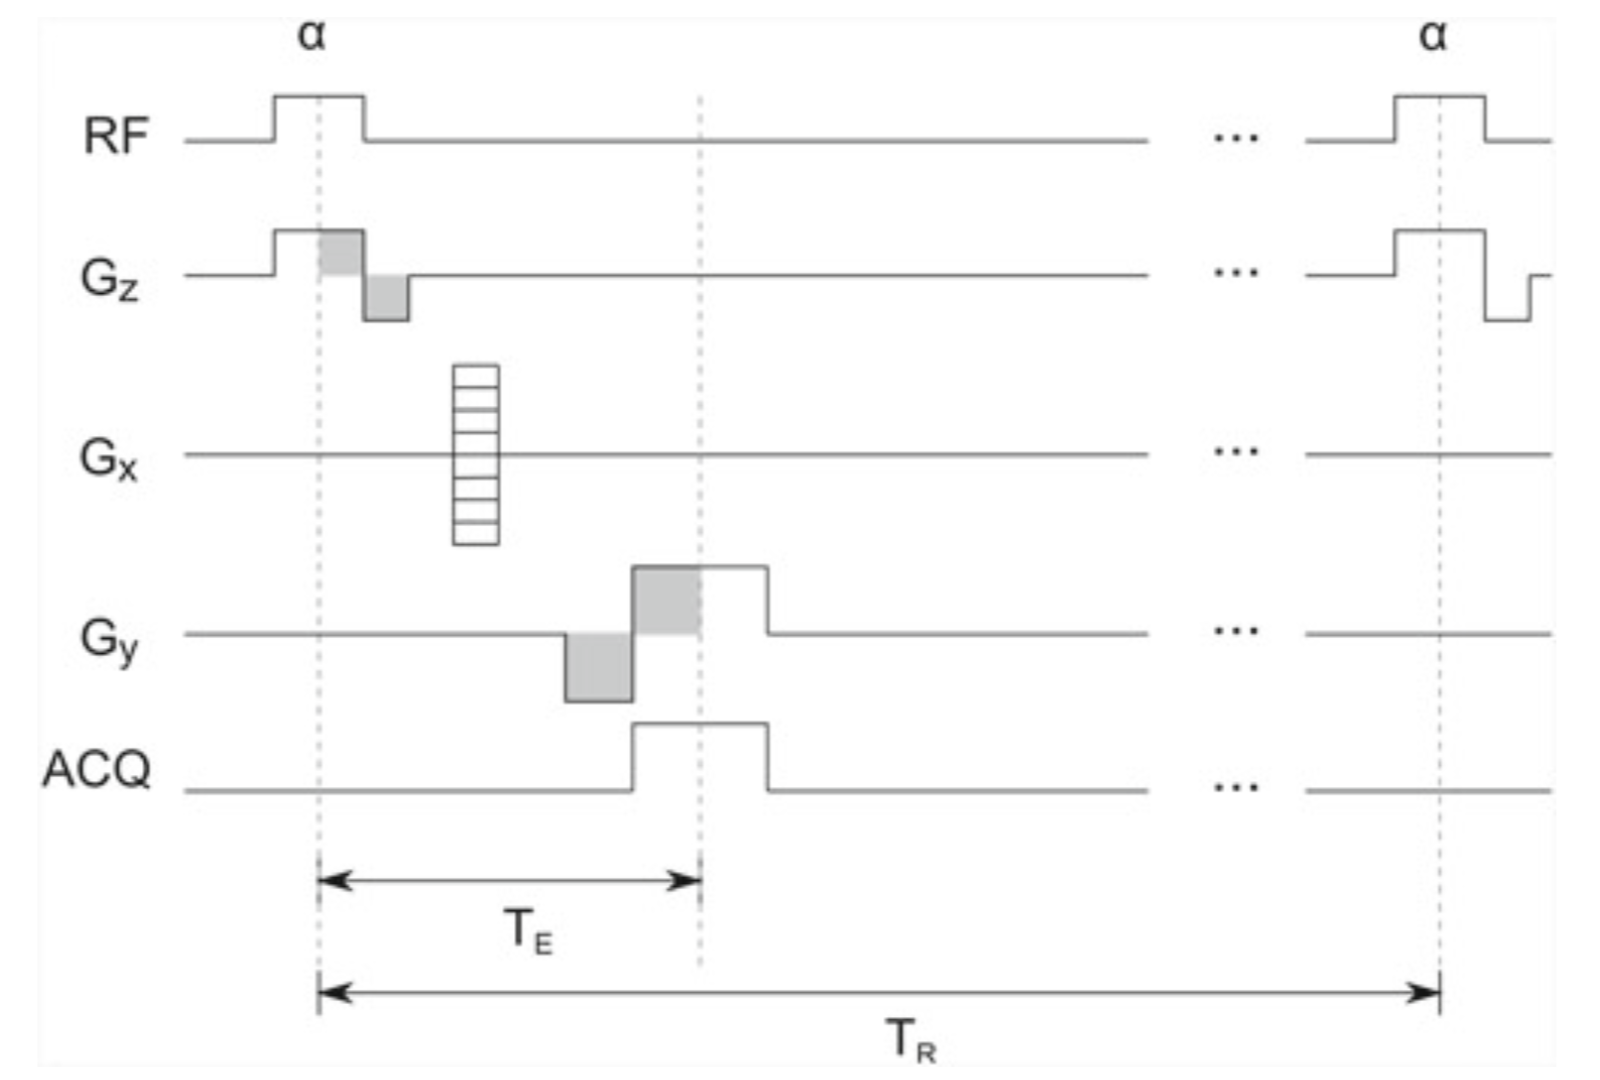
\includegraphics[width=0.9\textwidth]{img/intro/ge.png}}
\caption{梯度回波序列。此图来自文献\cite{haidekker2013medical}。}
\label{fig:ge}
\end{figure}
临床中所得到的MR图像大部分都是通过这两种回波序列的改进或者组合而得到,因此它们在MR成像中有着重要的作用。

\subsection{本节小结}
在这一节中,我们主要介绍了MR成像的基本概念并推导了其数学模型。MR成像可看成从k-space中采集数据并重建图像的过程,而不同的采样方式会对重建图像有着不同的影响,重建算法也会有所不同。MR序列是MRI中的重要概念,序列的参数,如偏转角、相位角、重复时间和回波时间等,会对重建图像有着不同的影响。这些概念我们在后面的章节也要用到。

\section{扩展相图}
\label{sec:epg}
在这一小节中,我们简单介绍扩展相图(extended phase graph, EPG)的数学模型,详细的信息请参考文献\cite{weigel}。这有助于我们理解MRI中回波强度的计算和第\ref{chap:snapMRF}章中snapMRF的程序设计。

EPG是用来描述和理解磁化在不同MR序列中响应的有力工具。在EPG中,梯度场、射频场、驰豫等对磁化的作用都可以用矩阵的简单计算来实现,因此在传统MRI和MRF中有着广泛的应用。相比与使用传统的Bloch方程来理解磁化响应的方法,EPG可以快速并准确地量化回波强度,尤其当序列中存在多个梯度场时。

\subsection{配置状态矩阵}
EPG中的第一个重要概念是用配置状态(configuration states)来表征梯度场使磁化失去相位和获得相位的过程。对于一个处于非中心位置$\textbf{r}$的等色子,其受到的磁场$\textbf{M}$可分解为:
 \beq M_x(\textbf{r})=|\textbf{M}|\cos\left(\gamma\textbf{r}\cdot\int_0^t\textbf{G}(t')\,\mathrm{d}t'\right)=|\textbf{M}|\cos(\textbf{k} \cdot \textbf{r}),\eeq
 \beq M_y(\textbf{r})=|\textbf{M}|\sin\left(\gamma\textbf{r}\cdot\int_0^t\textbf{G}(t')\,\mathrm{d}t'\right)=|\textbf{M}|\sin(\textbf{k} \cdot \textbf{r}).\eeq
这里相位角$\phi(\textbf{r})=\int_0^t\gamma\textbf{G}(t')\cdot\textbf{r}\,\mathrm{d}t'$定义在给定时间$t$上,并且
 \beq \textbf{k}(t)=\gamma\int_0^t\textbf{G}(t')\,\mathrm{d}t'\eeq
为失相的阶数(order)。注意这里的阶数也就是上节说讨论的采样轨迹。将坐标从实数改变到复数,则上式变为:
 \begin{align}
 M_+(\textbf{r})&=M_x(\textbf{r})+iM_y(\textbf{r})\nonumber\\ &=|\textbf{M}|e^{i\phi(\textbf{r})}=|\textbf{M}|e^{i\textbf{k} \cdot \textbf{r}}=(M_-)^*,
 \end{align}
 \begin{align} M_-(\textbf{r})&=M_x(\textbf{r})-iM_y(\textbf{r})\nonumber\\ &=|\textbf{M}|e^{-i\phi(\textbf{r})}=|\textbf{M}|e^{-i\textbf{k} \cdot \textbf{r}}=(M_+)^*.\end{align}
这里$^*$表示共轭。通过这样的坐标转换可以更加有效的表征水平磁化。

由于在一个体素中可能会包含多个等色子,而不是单一的,在实际计算中,我们需要考虑所有等色子的影响。将FOV内的水平磁化进行积分得到:
\begin{align} \tilde{F}_+(\textbf{k})=&\int_{\mathrm{FOV}}M_+(\textbf{r})e^{-i\textbf{k} \cdot \textbf{r}}\mathrm{d}^3r \nonumber\\ &\Longleftrightarrow M_+(\textbf{r})=\int_{\mathrm{FOV}}\tilde{F}_+(\textbf{r})e^{i\textbf{k} \cdot \textbf{r}}\mathrm{d}^3k,\end{align}
 \begin{align} \tilde{F}_-(\textbf{k})=&\int_{\mathrm{FOV}}M_-(\textbf{r})e^{i\textbf{k} \cdot \textbf{r}}\mathrm{d}^3r\nonumber\\ &\Longleftrightarrow M_-(\textbf{r})=\int_{\mathrm{FOV}}\tilde{F}_-(\textbf{r})e^{i\textbf{k} \cdot \textbf{r}}\,\mathrm{d}^3k.\end{align}
 这个方程表明由梯度场导致的失相可以由配置状态$F_+$和$F_-$来解释,因此所有等色子的状态也可以很容易地计算。

\subsection{分区状态方法}
EPG模型中第二个重要的概念是分区状态(partition state)方法,用于描述射频场对于磁化的影响。根据Bloch方程,射频场对磁化$[M_+,M_-,M_z]$的作用可以被定义为:
 \beq 
  T_x(\alpha)=
  \left[
  \begin{matrix}
   \cos^2\frac{\alpha}{2} & \sin^2\frac{\alpha}{2} & -i\sin\alpha \\
   \sin^2\frac{\alpha}{2} & \cos^2\frac{\alpha}{2} & i\sin\alpha \\
   -\frac{i}{2}\sin\alpha & \frac{i}{2}\sin\alpha & \cos\alpha
   \end{matrix}
   \right]
   \label{equ:alpha}
 \eeq 
和
 \beq 
  T_z(\phi)=
  \left[
  \begin{matrix}
   e^{i\phi} & 0 & 0 \\
   0 & e^{-i\phi} & 0 \\
   0 & 0 & 1
   \end{matrix}
   \right],
   \label{equ:phi}
 \eeq
 其中$\alpha$是偏转角,$\phi$是相位角。将方程(\ref{equ:alpha})和方程(\ref{equ:phi})经过以下变换
 $$T_\Phi(\alpha)=T_z(\Phi) T_x(\alpha)T_z(-\Phi),$$
 可以得到初始相位为$\Phi$的射频场对磁化的作用矩阵,我们用$T$来表示:
\begin{align} 
 \left[
  \begin{matrix}
   M_+ \\
   M_- \\
   M_z
   \end{matrix}
   \right]^+
   =&
   \left[
  \begin{matrix}
   \cos^2\frac{\alpha}{2} & e^{2i\Phi}\sin^2\frac{\alpha}{2} & -ie^{i\Phi}\sin\alpha \\
   e^{-2i\Phi}\sin^2\frac{\alpha}{2} & \cos^2\frac{\alpha}{2} & ie^{-i\Phi}\sin\alpha \\
   -\frac{i}{2}e^{-i\Phi}\sin\alpha & \frac{i}{2}e^{i\Phi}\sin\alpha & \cos\alpha
   \end{matrix}
   \right] \nonumber\\
   & \times
   \left[
  \begin{matrix}
   M_+ \\
   M_- \\
   M_z
   \end{matrix}
   \right]^-.
   \label{equ:transition}
 \end{align}
这里``$-$''和``$+$''的意思是在射频场作用之前和之后。方程(\ref{equ:transition})给出了射频场对于单一等色子的作用。在射频场的作用之后,磁化可以分为三个部分,即失相部分 ($M_+$), 得相部分 ($M_-$) and 垂直部分 ($M_z$)。

将配置状态矩阵和分区状态方法结合起来,就可以得到射频场对状态矩阵的作用:
 \begin{align}
 \left[
  \begin{matrix}
   \tilde{F}_+(k) \\
   \tilde{F}_-(-k) \\
   \tilde{Z}(k)
   \end{matrix}
   \right]^+
   =&
   \left[
  \begin{matrix}
   \cos^2\frac{\alpha}{2} & e^{2i\Phi}\sin^2\frac{\alpha}{2} & -ie^{i\Phi}\sin\alpha \\
   e^{-2i\Phi}\sin^2\frac{\alpha}{2} & \cos^2\frac{\alpha}{2} & ie^{-i\Phi}\sin\alpha \\
   -\frac{i}{2}e^{-i\Phi}\sin\alpha & \frac{i}{2}e^{i\Phi}\sin\alpha & \cos\alpha
   \end{matrix}
   \right]\nonumber \\
   & \times \left[
  \begin{matrix}
   \tilde{F}_+(k) \\
   \tilde{F}_-(-k) \\
   \tilde{Z}(k)
   \end{matrix}
   \right]^-.
 \end{align}
 这里
 \begin{align} 
 \tilde{Z}(k)=&\int_{\mathrm{FOV}}M_z(\textbf{r})e^{-i\textbf{k} \cdot \textbf{r}}\mathrm{d}^3r\nonumber\\ &\Longleftrightarrow
 M_z(\textbf{r})=\int_{\mathrm{FOV}}\tilde{Z}(k)e^{i\textbf{k} \cdot \textbf{r}}\mathrm{d}^3k.
 \end{align}
 
 \subsection{其他因素的作用}
 在以上两个部分,我们推导了射频场对磁化的作用矩阵$T$。除了射频场的作用,EPG模型也可以很容易地表示其他因素对磁化的作用,比如梯度场、驰豫等。这也是EPG模型的优点之一。
 
 由于梯度场造成的水平失相可以用平移矩阵$H$来表征:
 \beq H(\Delta k):\quad\tilde{F}_k\rightarrow\tilde{F}_{k+\Delta k} \quad\mathrm{and} \quad \tilde{Z}_k\rightarrow\tilde{Z}_k,\eeq 
 这里$\Delta k=\gamma\int_{t'=0}\textbf{G}(t')\mathrm{d}t'$。
 
 驰豫作用可以由下面的驰豫算子$E$实现。对于对于$k\neq 0$的状态:
  \begin{align}
 E&=
  \left[
  \begin{matrix}
   {E}_2 & 0 & 0 \\
   0 & {E}_2 & 0 \\
   0 & 0 & {E}_1
   \end{matrix}
   \right] \nonumber\\ &=
   \left[
  \begin{matrix}
   e^{-\tau/T_2} & 0 & 0 \\
   0 & e^{-\tau/T_2} & 0 \\
   0 & 0 & e^{-\tau/T_1}
   \end{matrix}
   \right].
 \end{align}
  这里$\tau$是驰豫进行的时间长度。当$k=0$时,需要在$\tilde{Z}(0)$上进行额外的$T_1$驰豫,方程变为:
 \begin{align}
 \left[
  \begin{matrix}
   \tilde{F}_+(k) \\
   \tilde{F}_+(-k) \\
   \tilde{Z}(k)
   \end{matrix}
   \right]^+
   =&
   \left[
  \begin{matrix}
   {E}_2 & 0 & 0 \\
   0 & {E}_2 & 0 \\
   0 & 0 & {E}_1
   \end{matrix}
   \right] \left[
  \begin{matrix}
   \tilde{F}_+(k) \\
   \tilde{F}_+(-k) \\
   \tilde{Z}(k)
   \end{matrix}
   \right]^- \nonumber\\
   & +
   \left[
  \begin{matrix}
   0 \\
   0 \\
   M_0(1-E_1)
   \end{matrix}
   \right].
 \end{align}
 
 \subsection{最终模型}
 到现在为止,我们已经定义了射频场的作用矩阵$T$,梯度场的失相矩阵$H$以及驰豫矩阵$E$。那么对于一个给定的MR序列,磁化在其中的相应可以表示为:
 \beq \Gamma(t)=\cdots E\cdot H\cdot T\cdot E\cdot H
 \cdot T \cdot \Gamma\ (t=0),\eeq 
 其中状态矩阵按照以下形式存储:
 \beq 
 \Gamma=
 \left[
  \begin{matrix}
   \tilde{F}_0 & \tilde{F}_1 & \tilde{F}_2 & \tilde{F}_3 & \tilde{F}_4 & \cdots \\
   \tilde{F}^*_0 & \tilde{F}^*_{-1} & \tilde{F}^*_{-2} & \tilde{F}^*_{-3} & \tilde{F}^*_{-4} & \cdots  \\
   \tilde{Z}_0 & \tilde{Z}_1 & \tilde{Z}_2 & \tilde{Z}_3 & \tilde{Z}_4 & \cdots
   \end{matrix}
   \right].
 \eeq 

\subsection{本节小结}
在小节中,我们简单回顾了EPG模型,并推导了射频场、梯度场以及驰豫对于磁化的作用矩阵。注意这里我们只给出了这三种因素的作用,但EPG模型也可以加入其他因素的影响,如扩散和运动。

\section{本章总结}
在本章节中,我们首先回顾了MR成像的基本原理和数学模型,并介绍了一些基本概念,如射频场、梯度场、驰豫、序列等。这有助于我们理解基于压缩感知的MR成像模型。之后我们简单回顾了扩展相图模型,并推导了射频场、梯度场和驰豫对于磁化的作用矩阵。这有助于我们理解第\ref{chap:snapMRF}章的程序设计。














